\subsection{Логотип как форма выражения массового сознания}
\label{1.3}

В 2000 году канадская журналистка и общественная активистка Наоми Кляйн
издала книгу под названием <<No Logo>>, сразу же окрещенную газетой
The New York Times <<евангелием антикорпоративного движения>>. В книге Кляйн дает
развернутую критику глобализации и современного экономического порядка в мире.
По ее мнению, мир, опутанный сетями глобальных брендов, лишен возможности свободного
выбора и не может полноценно развиваться.
Логотип-знак, как это уже бывало в истории,  попадая в бурную стихию общественных
страстей, неожиданно получает статус своеобразной эмблемы глобального <<зла>>.
Напрашивается аналогия с быком, которому показывают красную тряпку. Однако быки,
вопреки популярному представлению, совершенно не различают красного цвета,
а раздражают быка на арене совсем не красный цвет одежды матадора и мулеты,
a угрожающие движения, как ткани, так и самого матадора.
\emph{Лого} (неформальный вариант термина \emph{логотип} в разговорной речи),
как и мулета, есть всего лишь орудие, средство достижения цели,
но никак не поведенческий мотив.

Но в отличие от мулеты, логотип -- это комплексный изменчивый знак, значение и
функции которого, мы попробуем показать, могут существенно видоизменяться по мере
его врастания в массовое сознание современного общества. Иначе говоря, мы, в
отличие от Н.~Кляйн, выдвигаем слоган <<Know Logo>>. Сначала уточним свои исходные
позиции.

Справедливости ради следует отметить, что в самом начале книги, Кляйн объясняет,
что  ее название изначально не задумывалось как прямой лозунг <<Нет логотипам!>> или
же <<Долой логотипы!>>. Цель ее работы -- информировать своего читателя о деятельности
транснациональных корпораций и раскрыть секреты товаров, выпускаемых
под известными марками.\autocite{klein2003}
Получается, что <<лого>> привлекателен для автора только разве что стилистической
выразительностью и благозвучием (ассонанс и два сонорных согласных) формы слова.
Или, возможно, как легкий каламбур вокруг другого термина \emph{No Name} --
название товаров, не имеющих логотипа.  Но логотип, в некотором смысле, и есть
один из таких секретов. Кляйн в своей книге не придала этому значения.

\subsubsection{Видовые характеристики и знаковые параметры логотипа}

Мы исходим из представления, что логотип -- это знак визуальной коммуникации и
как таковой он:
\begin{enumerate*}
\item является технологическим расширением механизмов социальной адаптации
  естественного языка, в первую очередь родного языка;
\item как и любая коммуникативная технология он ориентирован на ускорение
  процесса коммуникации;
\item точно так же как и слово в речевом общении, он получает свое реальное
  значение и смысл только в акте коммуникации в рамках конкретной
  семиотической системы, в конкретной социокультурной ситуации.
\end{enumerate*}

Мы также исходим из представления, что логотип -- это знак социокультурной
коммуникации и как таковой он решает задачи символического обозначения границ
влияния владельца:
\begin{enumerate*}[label=\asbuk*)]
\item закрепление права собственности, принадлежности и владения;
\item персональная (само)идентификация и (само)реклама;
\item выражение социального статуса.
\end{enumerate*}

Наконец, самое очевидное: мы, разумеется, исходим из представления, что логотип --
это знак коммерческой коммуникации и как таковой он опосредует процесс взаимовыгодного
взаимодействия потребителя-покупателя с компанией-производителем товара. С него и начнем.

\paragraph{Товарный знак (торговая марка), бренд, логотип: разведение понятий}

%% TODO: вставить ссылки из реферата
В данной работе мы включаем логотип в категорию коммерческих знаков. В современном
маркетинге к ним относятся, в частности, товарный знак, торговая марка,
фирменное наименование, бренд, логотип, фирменный стиль, деловая репутация (goodwill).
Литература и публикации по данному вопросу дает весьма противоречивое
представление о их использовании \autocite{clifton2009}\autocite{eiri2011}\autocite{designing2009}\autocite{mollerup1999marks}\autocite{serov2005}\autocite{werkman1986}. Тем не менее, постараемся коротко зафиксировать их различие.

Все приведенные термины так или иначе делятся на
\begin{enumerate*}[label=\asbuk*)]
\item юридические, т.е. имеющие законодательное определение
  (это, например, товарный знак / торговая марка, фирменное наименование, гудвил) и
\item на термины, не урегулированные законодательством, но тем не менее
  используемые специалистами и общественностью.
\end{enumerate*}
Соответственно, использование таких терминов не имеет юридических последствий.
Возьмем из перечня только те, которые часто смешиваются  или объединяются с
понятием логотипа: товарный знак (торговая марка) и бренд и дадим им краткую
характеристику. Затем перейдем к логотипу.

\begin{itemize}
\item[Товарный знак.] Товарный знак (или торговая марка) на сухом
  экономическом языке является некоторым связующим звеном между производителем
  и массовым потребителем. Его основная задача -- привлечь внимания покупателя к
  товарам и дать ему возможность выбрать необходимые товары конкретного
  производителя. Появление знаков, представляющих производителя товаров,
  принято связывать с периодом становления товарно-денежных отношений, в то
  время, когда время мастеровые и ремесленники начали помечать свою продукцию --
  будь то кухонная утварь, предметы мебели и проч. -- знаками
  самоидентификации (клеймами). Так, известно, что в Российском законодательстве
  понятие товарного знака впервые получает свое определение  в 1767 году,
  с принятием Новоторгового Устава, содержащего правовые нормы,
  регулирующие внутреннюю и внешнюю торговлю\autocite{pantuhinaAM}.
  Схематично взаимосвязь товарного знака с интересами производителей и
  потребителей можно представить в виде схемы(см. рис.~\ref{fig:pantuhina}).
  \begin{figure}[h!]
  \centering
  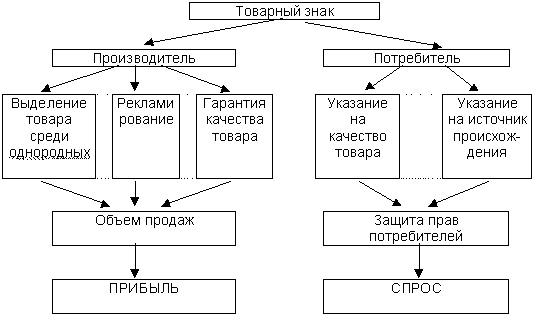
\includegraphics[width=.7\linewidth]{images/pantuhina}
  \caption{Взаимосвязь товарного знака с интересами производителей и потребителей}
  \label{fig:pantuhina}
\end{figure}

  Как видим, основная функция товарного знака -- помочь потребителю выделить
  товар или услуги соответствующего производителя из аналогичных товаров и услуг
  других производителей. Кроме этого, товарный знак дает возможность установить
  источник происхождения товара. Далее, товарный знак, ориентируя потребителя
  при выборе того или иного товара, тем самым становится своего рода гарантией
  качества товара. В этом его вторая функция. Поскольку выбор товара основывается
  на его ожидаемых свойствах, то следующую функцию товарного знака можно обозначить
  как информирование покупателя о наличие того или иного качества в данном товаре.
  Наконец, рекламирование можно также выделить в качестве еще одной функцию
  товарного знака. Иначе говоря, товарные знаки помогают стимулировать и
  сохранять спрос на товары конкретного производителя, тем самым обеспечивая
  широкую известность не только компании производителю, но и товару.

\item[Бренд.] Во второй группе -- это, пожалуй, самый яркий термин,
  сегодня более чем успешно конкурирующий с термином \emph{товарный знак} в
  средствах массовой информации, в публичном дискурсе и повседневном речевом
  общении, как в России, так и за рубежом. Высокая частотность употребления
  того или иного нового слова в практике речи, как известно, фактически
  сводит на нет любые попытки однозначно определить его содержание или значение.
  В переводе с английского <<brand>> обозначает: раскаленное железо, выжженное
  клеймо, фабричное клеймо, фабричная марка, а также выжигать клеймо и
  отпечатываться в памяти, оставлять неизгладимое впечатление.\autocite{oxford_dictionary}
  Исходя из буквального значения этого слова, очевидно, что оно,
  так же, как и \emph{товарный знак}, выполняет функцию индивидуализации товара,
  услуги, или компании производителя, с одной стороны. С другой, такой
  <<индивидуализированный образ>> должен прочно и надолго войти в долговременную
  память потребителя. Понятно, что при этом исполнение самой функции может
  периодически принимать несколько агрессивный характер, опираясь на
  суггестивные возможности знаков коммуникации, о которых мы говорили ранее.
  По факту, бренд, как правило, получает свое материальное воплощение
  в определенном слове, словесном выражении в комплексе со своим
  графическим выражением -- логотипом. В результате, брендом может быть
  наименование товара, услуги, фирмы, не зависимо от того, зарегистрированы
  они или нет. Более того, брендами в последнее время стали называть имена
  ярких исторических личностей, оставивших у нескольких поколений потомков
  неизгладимую память о себе, например: Петр I. Когда в 2002 году британец
  Саймон Анхольт, один из ведущих мировых специалистов в области маркетинга,
  предложил концепцию <<брендинга мест>>, через некоторое время начали
  появляться <<города-бренды>>, <<территории-бренды>>  и
  проч.\autocite{brending} Наконец, судя по последним публикациям по проблеме,
  брендом можно сделать и собственную личность.
  \autocite{peters1999brand}\autocite{schawbel2009me}\autocite{deckers2012branding}

  Более детально мы будем говорить о бренде позднее. А пока, в сжатой форме,
  и несколько опережая изложение, сформулируем его суть. Практика показывает,
  что сегодня каждый производитель мечтает превратить свой товарный знак в бренд.
  Очень упрощенно можно предварительно сказать, что термин \emph{бренд} обозначает
  некий
  привлекательный образ, сознательно и изощренно навязываемый  массовому человеку
  извне. В идеале, это образ, непроизвольно возникающий в сознании человека при
  восприятии определенного слова-образа (логотипа), способный формировать мысли,
  образ жизни и поступки человека в массовом обществе потребления. Исходя из
  практики применения этого термина, функцию бренда можно определить как
  формирование автоматических потребительских реакций человека, соматических
  маркеров, при восприятии определенного логотипа.

\item[Логотип.] Из сказанного выше, казалось бы, естественным образом вытекает
  представление о логотипе как вспомогательном знаке, графическом атрибутом бренда.
\end{itemize}

В тоже время, из практики известно, что многочисленные маркетинговые фирмы и
агентства считают логотип  ни больше ни меньше как краеугольным камнем рекламного
бизнеса и по этой причине требующим, помимо всего прочего, весомых финансовых
вливаний. Для примера: британское дизайнерское агентство Marque получило за
разработку логотипа очередных Игр Содружества в Глазго
(XX Commonwealth Games 2014)  \$ 95,000, а логотип для Олимпийских игр прошлого
года в Лондоне принес дизайнерской компании Wolff Ollins  \$ 625,000.
В 2008 году обновление логотипа обошлось компании Pepsi в \$ 1,000.000,
выплаченных дизайнерам фирмы Arnell Group. Логотип корпорации BBC (1997) --
\$ 1,800,000,  логотип консалтинговой компании Accenture (2001) -- \$ 100,000,000,
логотип британской нефтегазовой компании BP (1989) – \$ 210,000,000.\autocite{logotipy}
Каким образом обычный визуальный знак, будучи технически лишь оригинальным
начертанием наименования организации или товара \autocite[][65]{rogers2001marketing},
будучи элементарным средством идентификации -- становится эксклюзивным и
дорогостоящим товаром, мы и попробуем теперь разобраться. Для начала
абстрагируемся от живой социокультурной практики, в которой функционирует
логотип, и посмотрим на знак исключительно в его знаковых характеристиках.
Будем двигаться от общего к частному.

\subsubsection{Знаковые параметры логотипа}
Для удобства сформулируем методологическую матрицу для дальнейшего
рассуждения, обобщив базовые аксиомы знака. Для этого обратимся к
работе А.Ф. Лосева <<Знак. Символ. Миф>> \autocite[][32-42]{losev1982}, где он, в частности,
предлагает различать следующие аксиомы общей информации:
\begin{itemize}
\item[Аксиома 1.] \emph{Всякий знак предполагает, что существует нечто внезнаковое
    обозначаемое, и уж тем более нечто означаемое и значащее.} Действительно,
  в конце предыдущего параграфа мы утверждали, что для нас логотип -- знак
  реальный, т.е. если бы для него не было внезнакового объекта обозначения,
  то его нельзя было бы считать знаком. Устранение объекта или произвольный
  выбор объекта означали бы попросту выход из знаковой сферы во внезнаковую
  область.
\item[Аксиома 2.] \emph{Всякое обозначаемое и тем более означаемое предполагает,
    что есть знак, которым оно обозначено.} Иными словами, логотип есть не просто
  реальный, но объективно-реальный знак, а не просто абстрактная
  внутрипсихологическая игра понятий.
\item[Аксиома 3.] \emph{Всякий знак функционирует как акт обозначения для
    чего-нибудь обозначаемого и уж тем более для всякого означаемого.}
  Проблему с определением внезнакового предмета для логотипа в общем виде
  мы обозначили выше. Данная аксиома просто еще раз утверждает обязательность
  его наличия.
\item[Аксиома 4.] \emph{Всякий знак предполагает для себя того или иного
    внезнакового, но вполне специфического носителя.} Логотип, чтобы быть
  самим собой, т.е. иметь свои качества свойства, должен отличаться
  от всего того что им не является. В противном случае мы не могли бы
  говорить о его существовании вообще. Логотип получает свою специфику
  лишь при условии наличия внезнакового носителя, каковым будет
  материал из которого он изготавливается, равно как или материал или
  поверхность на которую он наносится.
\item[Аксиома 5.] \emph{Всякое обозначение требует для себя своего
    собственного и специфического, а главное, своего собственного внезнакового
    носителя.} В корпоративной среде конкретным носителем логотипа может быть,
  в частности, внутренняя документация компании, канцтовары,
  наружная реклама, веб-сайт, здание офиса и проч.
\item[Аксиома 6.] \emph{Всякий обозначаемый и уже тем самым всякий означаемый
    предмет необходимо требует для себя собственного и специфического, а
    главное, своего собственного внезнакового носителя.}
  Согласно данной аксиоме обозначить нечто -- значит признать, что это
  нечто существует. С другой стороны, обозначить нечто можно только тогда,
  когда это нечто существует. При этом само обозначенное -- в нашем случае
  логотипом -- может быть как глубоким, так и поверхностным, целостным и
  частичным, правильным и неправильным, т.е. может иметь разные способы и
  виды своего обозначения. Наличие общего внезнакового объекта или предмета,
  правильно или неправильно обозначаемого с разных сторон, делает сам
  факт обозначения реально существующим.
\item[Аксиома 7.] \emph{Всякий знак предмета есть смысловое отражение
    предмета.} Другими словами, обозначение действительно имеет место
  быть только в том случае, когда знак -- логотип, обозначаемое им и
  сам акт обозначения наполняются определенным смыслом и знак становится
  собственно смысловым знаком.
\item[Аксиома 8.] \emph{Соотношение между знаком и обозначаемым, кроме
    их фактического соотношения, находится еще и в состоянии смыслового
    взаимного самоотражения.}
\end{itemize}
Любой знак есть либо смысл, либо носитель смысла. При этом любое обозначаемое
есть тот предмет, который получил осмысленное содержание при помощи того или
иного осмысленного знака.

От общей аксиоматики перейдем к поиску адекватного осмысленного структурного
определения логотипа. Сначала рассмотрим общепризнанную  классификацию знаков
Ч.~Пирса: иконы, индексы и символы,  основанную на двух дихотомиях --
противопоставлении смежности и сходства, противопоставлении естественной
и произвольной связи.\autocite[322]{jakobson1985} Коротко о каждом.

\begin{enumerate}
\item Иконическими знаками называются такие знаки, у которых форма
  и содержание сходны структурно или качественно, т.е. означаемое
  и означаемое фактически подобны. Сам Пирс пишет: <<Иконический знак (icon)
  есть знак, отсылающий к объекту, который он обозначает, просто в силу
  своих свойств, которыми обладает независимо от того, существует ли
  вообще какой-нибудь Объект или нет. Верно, что пока в действительности
  нет такого Объекта, иконический знак не действует как знак.>> \autocite[][185]{jakobson1985}
  Например, рассуждает Пирс, план сражения или батальное полотно есть,
  по сути дела, иконические знаки, если считать их содержанием само сражение.
\item Индексом (index) (или индексальным знаком) называется знак, у которого
  форма и содержание смежны в пространстве или во времени.
  У Пирса мы читаем: <<Индекс есть знак, отсылающий к Объекту, который он
  обозначает в силу того, что он действительно подвергается воздействию
  этого Объекта. (\ldots) Поскольку Индекс подвергается воздействию
  Объекта, он необходимо имеет какое-то общее с этим Объектом Качество,
  и именно в соответствии с ними [качествами] он отсылает к Объекту.>> \autocite[][186]{jakobson1985}
  Например, отпечаток следа на песке, позволяющий сделать предположение о том,
  кто мог пройти в этом месте ранее, вид поднимающегося вверх дыма,
  предполагающий присутствие поблизости огня, ярко выраженные симптомы болезни,
  предполагающие протекание самой болезни, -- все это будут индексальные знаки.
  На самом деле, по-видимому, в данном случае правильнее было бы говорить не
  столько о традиционной смежности формы и содержания, сколько о
  причинно-следственных связях, возникающих между ними.
\item Наконец, символом (symbol) (или символическим знаком) называется знак,
  для которого связь между формой и содержанием формируется произвольно,
  по некоторому соглашению, касающемуся именно данного знака. В формулировке
  Пирса: <<Символ есть знак, который отсылает к обозначаемому им Объекту в силу
  закона, обычно -- ассоциации общих идей, действующего так, чтобы заставлять
  нас интерпретировать Символ как отсылающий к этому Объекту. Таким образом,
  он сам является общим типом или законом.>> \autocite[][186]{jakobson1985} И если для иконических
  и индексальных знаков форма дает возможность догадаться о содержании знака
  даже не знакомому с ним интерпретатору, то форма символических знаков сама
  по себе, т.е. вне специального договора, не  может дать  вообще никакого
  представления о их содержании.
\end{enumerate}

Следует отметить, тем не менее, что классификация Пирса не носит жесткий,
завершенный характер. Знаки подвижны и могут взаимопроникать друг в друга.
Сам Пирс признает, что, иконический знак может входить в состав индексального
знака, а индексальный знак может быть частью символа, <<хотя это и будет особым
Индексом>>, предупреждает Пирс. Такая подвижность знаков представляется
нам чрезвычайно важной. На самом деле, логотип с легкостью можно было бы
поместить в любую из трех категорий. Во-первых, он является индексальным знаком,
т.е. указывает на конкретного производителя товара или поставщика конкретных
услуг. Он также указывает на конкретную массу потребителей, на которых
ориентирован производимый товар или услуга. Во-вторых, логотип, как
элемент маркетинговой стратегии, может -- и даже должен -- становиться частью
символа, даже амальгама символов и в этом качестве указывать на имидж и
репутацию компании производителя, с одной стороны, и на сложное аффективное
целое позитивных потребительских ожиданий, эмоций и ассоциаций в связи с
деятельностью данного производителя, с другой. В этом случае, в массовом
сознании потребителей он, как <<особый индекс>>, начинает отождествляться
с брендом компании производителя. Наконец, логотип, естественным образом
включает в себя иконическую составляющую. На элементарном техническом уровне,
по форме исполнения, логотип является изображением, иконом, схематически
обобщающий направление деятельности своей компании. На смысловом,
символическом уровне, он лапидарно синтезирует философию компании,
под которой следует понимать ее желаемое представление о себе в сознании
массового потребителя. Иначе говоря, здесь мы имеем дело с функцией двойной
иконической сигнификации. Рассмотрим суть иконичности подробнее.

\subsubsection{Иконичность логотипа}

\textbf{Философский аспект}

%% TODO: разметить библиографические ссылки.
Исторически, идея изобразительной природы знаков, т.е. представление о знаках
как изобразительных подобиях обозначаемых ими объектов, встречается уже в
одном из сократических диалогов Платона, где собеседники делают предположение о
том, что <<имя тоже в некотором роде есть подражание, как и картина>>.\autocite{kratil2013} В
отличие от картины, тем  не менее, знаки здесь понимаются как подражания внутренним свойствам и
качествам вещей. Среди изображений наиболее близки знакам (в узком смысле слова), по-видимому,
рисунки, которые по способу начертания и по своему происхождению родственны знакам письма. Их
родственная связь, в частности, зафиксирована в самой этимологии слова <<знак>>, <<рисунок>>,
<<чертеж>> в разных языках*, утверждая прежде всего их сходство в нанесении каких-то видимых отметок на
плоскости. Примечательно, что родство рисунка с другими знаками может распространяться не только на
видимую форму, но и на невидимое содержание, чему свидетельствуют комментарии мастеров и теоретиков
эпохи Возрождения.\autocite[][527-535]{zukarro1981} Внутренняя форма, или <<внутренний
рисунок>> предмета здесь символизируется, становится идеальным образом первообоазной сущности (идеи),
иначе: божественного первообраза. (* Например, в английском: <<sign>> и <<design>>, в немецком –
<<Zeichen и Zeichnung>>,  в русском – <<знаменить>>, т.е. наносить рисунок на иконе (однокоренное со
словом <<знамение>>, <<знамя>>, этимологически близкое термину <<знак>> \autocite[][140]{chertov1993}

%% TODO: что за Чертов?
В крайнем выражении, например, в христианской иконографической традиции
символ и изображение уже полностью отождествляются со своим праобразом,
как подчеркивает, например, П.А.~Флоренский.\autocite{florensky1995}
В результате, постепенно складывается традиция, согласно которой любое
изображение начинает рассматриваться как нечто обладающее большей достоверностью,
чем условный, конвенциональный знак. Более того, изображению начинают
приписывать <<статус документального свидетельства подлинности изображаемого>>.
(Чертов, с. 143) В первую очередь, конечно же, <<иконе>>, появившейся в
христианском искусстве как продолжение давней традиции фиксировать документально
образ умершего. \autocite{lihachev1971}
Парадоксально, но, если иконопочитатели раньше видели в них прямое подтверждение
реальности изображенных объектов культа, то иконоборцы, для которых изображение
как таковое также являлось достоверной копией, напротив,  оспаривали саму
<<возможность документально зафиксировать в иконе вид умопостигаемого божества>>
(Чертов, с.143). Соответственно, для последних изображения на иконах были
всего лишь кощунственными идолами. Компромиссная точка зрения, в конце
концов, восторжествовала: изображение на иконе -- подлинное свидетельство
неизменной внутренней сущности изображаемого, а не случайных внешних
моментов.\autocite[][18]{lasarev1986, bichkov1989}

Должно быть понятно, что большая достоверность изображения по сравнению с
конвенциональным знаком свойственна не только религиозному или
мифологическому сознанию прошлого. Ведь мифологическое сознание в современной
культуре по-прежнему руководствуется теми же самыми представлениями.
Мы как бы <<забываем>> в некоторых случаях, что изображение и изображаемое
совсем не одно и то же. Скажем,
телевизионное изображение того или иного человека рутинно воспринимается
как сам этот человек, а не как знак. Против такого забывания, в
сущности, направлен и интеллектуальный протестный пафос критиков современного
общества потребления, о чем мы говорили ранее. Общества, покупающего себе образы
(shopping for images).\autocite{ginsberg1984supermarket} Для нас же здесь вопрос о
достоверности конвенциональных знаков и изображений лежит в плоскости аналогии.
Ошибочные, ложные или просто фантастические представления, как мы знаем по
рекламе, могут в равной степени легко передаваться как знаками, так и
изображениями. Скажем, сам факт изображения Снегурочки вряд ли покажется
достаточным основанием для признания ее реальности. Как знаки, так и
изображения -- это средства коммуникации, и как таковые они способны в равной
степени передавать достоверные и недостоверные сведения. Именно на основании
общности коммуникативных и репрезентативных функций изображений и условных знаков
Ч.~Пирс включает изображения в  свой знаковый триптих.

Все это пока лишь самое общее обсуждение иконичности, имеющее отношение
к логотипу лишь постольку, поскольку в плане выражения он  является иконическим
знаком и, в свете сказанного выше, также может получать двойственное
истолкование. Однако поменяем  фокус анализа.

\textbf{Психологический аспект}

В посмертно опубликованной работе
<<Экзистенциальные графы>> Пирс также пишет: <<Бытие иконического знака принадлежит
прошлому опыту. Он существует только как образ в памяти>>.
(Цит.~по:~\autocite{jakobson1983}) То есть речь идет о припоминании или
узнавании общих качеств и свойств узнаваемого объекта. Но именно эту общность
свойств и качеств знака и объекта ставит под сомнение У.~Эко, для которого
отношение иконического знака к реальному объекту лежит за пределами собственно
семиотических отношений. По его представлению иконический знак также условен,
как и конвенциональный знак. Подобно <<автоматизированному рефлексу>>  он
воспроизводит лишь некоторые общие условия восприятия объекта, и их сходство
определяется ментальной репрезентацией, перцептивной моделью, вызываемой
объектом в психике субъекта. В знаке отображается не то, что видит художник,
а только то, что он знает о видимых, предполагаемых и конвенциональных свойствах
и качествах предмета. <<Иконические знаки, -- считает Эко -- воспроизводят
некоторые условия восприятия объекта, но после отбора, осуществленного на
основе кода узнавания, и согласования их с имеющим репертуаром графических
конвенций>>\autocite[][160]{eko1998} Иначе говоря, для распознания
изображения мы используем данные о знакомых, виденных вещах и явлениях, которые
хранятся в долговременной памяти в качестве неких эталонов.  Как и в случае с
восприятием речи, распознавание изображения делается возможным благодаря коду
узнавания, который вычленяет отдельные существенные черты предмета для хранения
в памяти и дальнейшего использования в коммуникации. Так, например, мы можем
издалека распознать зебру и даже воспроизвести ее на рисунке, опираясь лишь на
две наиболее существенные черты: полосатость и четвероногость, абстрагируясь от
остальных подробностей ее анатомии. Причем функционирование кодов узнавания
(как и кодов восприятия), полагает У.~Эко, в значительной степени детерминировано
культурным фоном, или точнее -- конвенцией визуальной репрезентации в различных
культурах. Если для нашего культурного мировидения  зебра экзотична и необычна
по сочетаемости полосатости и четвероногости, то, скажем, для кенийского
африканского племени, промышляющего охотой на зебр, значимыми могут оказаться
совершенно иные свойства.\autocite[][160]{eko1998}

Примечательно, что семиотические интуиции У.~Эко, с одной стороны, перекликаются
с отечественной психологической теорией знака, о которой мы говорили ранее,
с другой,  находят свое подтверждение в том числе и в результатах современных
нейро-исследований физиологии зрительного восприятия человека. Исследователи,
в частности, утверждают, что представление о наличии оптического образа,
передаваемого глазного яблока на экран -- зрительную кору головного мозга --
очевидное логическое заблуждение. Для нейрофизиолога человек -- в высшей степени
визуальное существо, в том смысле, что у него в задней части головного
мозга функционируют тридцать зрительных полей, позволяющих ему видеть мир.
Каждая из этих зон, как показывают исследования, вероятно отвечает за разные
аспекты зрения.\autocite{velyanur2006}

Поэтому для понимания зрительного восприятия необходимо <<забыть про идею образа
в мозгу, а вместо этого подумать о преобразовании или символическом
представлении объектов и событий во внешнем мире.>> \autocite[][33-34]{velyanur2006}
Точно также как знаки письменности представляют или символизируют нечто,
чем они не являются физически, так и воспринимаемые нами события и предметы
внешнего мира являются результатом активности нервных клеток мозга и
разнообразных примеров их работы. При такой постановке вопроса нейрофизиологи
становятся своего рода дешифровщиками, пытающимися <<взломать чужой код>>,
т.е. <<код, который использует нервная система для изображения внешнего мира.>>\autocite[][34]{velyanur2006}
Иными словами, нейрофизиологи тоже становятся семиотиками.

Два важных следствия для понимания иконичности логотипа:
\begin{enumerate}
\item Его изобразительность есть отражение лабильности внутренней
  психической жизни (деятельности мозга) дизайнера -- его создателя, в одном
  случае, и воспринимающего (смотрящего на него) реципиента, в другом.
\item В обоих случаях восприятие апперцептивно и обусловлено культурным
  контекстом, в широком смысле слова.
\end{enumerate}

\textbf{Прагматические аспекты логотипа.}

Новый прагматический подход к описанию знаков и знаковых систем предложил
современный израильский филолог и семиотик А.Б.~Соломоник.
\autocite{solomonik1995}\autocite{solomonik2004}\autocite{solomonik2009}
В частности, он предложил классифицировать знаковые системы по принципу
эволюционного развития и на основе образующего их базисного знака.
Все существующие знаковые системы иерархически распределились по пяти типам и
по пяти видам знаков с нарастающей степенью абстрактности: естественный знак,
образ (имидж), слово, иероглиф, символ с постоянным значением, символ с
переменным значением.\autocite[][76-86]{solomonik2009} Так как мы не имеем
никакой возможности рассмотреть здесь все классификацию целиком, мы
ограничимся лишь обозначением направления классифицирующей мысли автора
концепции и кратким описанием  базовых знаков трех первых уровней.

Естественные знаки -- осязаемые предметы или явления природного происхождения,
представляющие другой предмет или явление. Так, следуя логике <<если \ldots, то\ ldots>>,
по лужам мы можем судить о прошедшем дожде, по свету от лампы о том,
что нужный нам человек возможно еще не спит и т.д. Соломоник называет их
<<первыми в истории знакового взаимодействия между природой и человеком>>.\autocite[][78]{solomonik2009}
Над ними надстраиваются уже знаки, придуманные человеком, и в первую очередь --
образы. Точно так же как образное мышление приходит сразу вслед за
манипулированием предметами в развитии маленьких детей и перед стадией
овладения языком, образ как базовый знак нового уровня надстраивается над
естественным знаком и его системами, взаимодействуя с ними, вбирая и представляя
их по-новому. Знак-образ уже не является реальным предметом. Это изображение
чего-то из реальности, связанного с ним отношением, близким к изоморфизму,
т.е. по наличию точек совпадения по конструкции и/ли по содержательным
компонентам. Совпадения <<либо по существу, либо по внешнему виду, либо по
ассоциациям, вызываемым образом и изображаемым>>.\autocite[][52]{solomonik1995}
Этот тип, соответственно, включает в себя очень большое количество
знаковых систем -- ориентировочных, рисуночных, игровых и проч.
Наконец, следующая стадия в развитии человека (и человечества),
приходящая после овладения началами образного представления -- шифрование
окружающей реальности при помощи слов языка. Слова уже существенно абстрактнее
знаков-образов по причине значительной произвольности и удаленности от
своего референта.

Остановимся здесь. Пожалуй, главное в систематизирующей мысли А.Б.~Соломоника:
<<каждый переход от одного базисного знака к другому сопровождается изменением
объема шифрующейся в одном знаке действительности>>.\autocite[][79]{solomonik2009}
Естественный знак шифрует данный предмет в каждом конкретном случае, образ
уже начинает стремиться к родовому обобщению, в то время как основная
масса слов -- это коллективные понятия. Посмотрим более внимательно на категорию
знака-образа, своего рода прагматическую альтернативу икону Ч.~Пирса.

Любой знак-образ изначально материализуется в виде реальных предметов.
Если положить часы в витрину магазина, то это будет естественный знак того,
что здесь продаются часы. В то же время нахождение часов в витрине делает
этот знак в некотором степени образным, поскольку они представляют не только
те конкретные часы, которые продаются в данный момент, но продажу часов вообще.
То есть знак-образ призван представлять все аналогичные предметы данной группы.
Нарисованные часы на витрине магазине становятся знаком в полном смысле слова,
хотя только знаком-образом. Если же на вывеске магазина написать <<Часы>>,
то это будет знаком языкового кода, который, по сути дела, будет выполнять
ту же самую функцию, что и нарисованные часы, равно как и настоящие часы в
витрине. А если к яркому изображению на вывеске магазина добавить логотип
знаменитой часовой компании, то образ сразу же приобретает символический
характер, свойственным формализованным символическим системам в классификации
А.Б.~Соломоника.

Одни знаки-образы в большей или меньшей степени внешне похожи на реальный референт.
В этом случае речь идет о знаках-<<иконах>>, распространенных в практической жизни
гораздо больше остальных знаков <<просто потому, что вследствие своей похожести на
изображаемое они понятны всем категориям пользователей и не умеющим читать и даже
не знающим языка страны, где они находятся.>> \autocite[][55]{solomonik1995}
Так, рисунок ботинок на вывеске достаточно ясно указывает на магазин обуви или мастерскую по
ремонту обуви. Понятно, что чем популярнее изображаемый объект в мире -- скажем,
продукты питания -- тем быстрее распознается изображение. В других случаях культурная
традиция данного общества и даже местные обычаи ограничивают понятность даже
самых отчетливых <<икон>>. Более того, иногда -- даже в пределах одной страны -- для
одного изображаемого могут использоваться разные <<иконы>>. Варьирование достигается
преимущественно за счет использования разных тропов -- часто метонимии и синекдохи --
для построения образа. Например, нарисованный конверт -- простой пример знака, обозначающего почту.
К универсальным системам, построенным преимущественно на иконах, относится система
дорожных знаков. \autocite[][56-58]{solomonik1995} Логика такой системы достаточно
примитивна, поскольку каждый знак в ней оценивается по отдельности и в каждой
конкретной ситуации.

Другие знаки-образы ковенциональны, т.е. исключительно условны и произвольны
по обозначению вложенных в них идей сходства между изображаемым и его символикой.

Например, на гербе Российской Федерации изображен двуглавый орел,
отражающий силу и мощь государства, символ союза светской верховной власти  и власти духовной.
Изоморфизм здесь, казалось бы, практически равен нулю. Но только по
схожести внешних признаков. Иначе говоря, он уступает место внутреннему изоморфизму:
<<по связи образа с изображаемым через представляемые или культурно-обусловленные
символы>>. \autocite[][61]{solomonik1995} В исторической перспективе, по мере
усложнения форм социокультурной практики жизни, человеку уже недостаточно просто
регистрировать происходящее и знаки-образы получают дополнительную смысловую нагрузку,
чтобы передавать сложные внутренние связи между предметами и свое отношение к изображаемому.
Реалистичный знак-образ начинает все больше тяготеть к синтетическому визуальному обобщению
и новому статусу образа-символа. Соответственно, нарастает и степень его абстрактности.
Чем выше степень абстрактности знака и чем слабее его связь с обозначаемым
референтом, тем легче оперировать им внутри знаковой системы: образовывать
сложные знаки из базисных, составлять сложные выражения из простых знаков, давая
им большую степень свободы и новые эвристические возможности и качества.
И последнее: получающийся сложный образ, как,  впрочем,  и образ вообще, невозможно
разложить на простые составляющие компоненты, что, в свою очередь, <<не дает нам
возможности подключить при восприятии разум; мы вынуждены реагировать
эмоционально.>> \autocite[][77]{solomonik1995}

Думается, подход А.Б.~Соломоника имеет несколько преимуществ перед трехчленной
схемой Ч.~Пирса. Во-первых, здесь распределение знаков происходит по
иерархическому принципу, последовательно и в нарастающем порядке. Во-вторых,
в основу классификации положен единый критерий степени абстракции знаков,
позволяющий наглядно представить динамику постепенного отдаления знака от
своего референта и обретения им расширяющихся синтаксических возможностей в ту
систему, куда он включается. В-третьих, каждый вышестоящий знак в иерархии
приобретает дополнительные возможности охватывать все большие сегменты реальности,
которые он шифрует.

Соответственно, в этом плоскости рассуждения логотип у нас переходит из категории
индексов Пирса, которым при данном подходе соответствуют естественные знаки,
в категорию знаков-образов, первых собственно знаков с потенцией обобщения и
интериоризации опыта. Из двух описанных выше потенций быть  образом-иконом
или конвенциональным образом-символом, мы определяем логотип в категорию
образов-символов. В следующем пункте мы поместим логотип в социокультурный
контекст и рассмотрим предпосылки и генезис его символической эволюции.
Но сначала обобщим сказанное:
\begin{enumerate}
\item По функциональному назначению логотип есть коммерческий знак-образ.
\item По своей способности обобщения логотип есть эвристический знак-символ.
\item По своей способности отражения сегментов реальности логотип конвенционален и условен.
\item По факту психического отражения логотип воспроизводит соотношения схемы
  взаимодействия перцептивных и апперцептивных факторов в сознании дизайнера-изготовителя
  и реципиента-потребителя.
\end{enumerate}

\subsubsection{Символичность логотипа}
По словам П.А.~Флоренского: <<Основание символики -- самая
реальность>>.\autocite[425]{book:florensky1} В повседневном речевом общении и прикладной
деятельности под символом (от греч. <<знак, опознавательная примета>>) обычно
понимается графическое изображение знака, буквы, предмета, действия или явления.
В философии и гуманитарных науках символ это любой предмет или явление,
пластический или словесный образ, который какой-то смысл, т.е. личностную ценность,
как мы подчеркивали раньше. Понимаемый таким образом символ указывает на значимость,
ценность данных предметов, явлений и проч. как для отдельной личности
(индивидуальные личностные символы), так и для малых и больших, массовых групп,
в том числе народов, государства, человечества в целом. Так, голубь и изображения
голубя могут восприниматься как мировой символ ценности, значимый для всего
человечества.

Символическая ценность логотипа, разумеется, не имеет масштабов общечеловеческой ценности.
В то же время его массовое присутствие в повседневной практике жизни в современном
обществе позволяет назвать его феноменом поистине мирового масштаба. Реальность
бытия логотипа, в которой раскрываются его символические качества -- как в его графическом
воплощении, так и в его идейности - образует своеобразный континуум.
Крайние полюса этого континуума оформляет один и тот же детерминант -- бренд.

\paragraph{Социокультурный генезис логотипа}

В самом начале параграфа мы говорили, что логотип решает задачи закрепления права
собственности, идентификации и выражения социального статуса обладателя.
Последовательно расширим этот тезис.

% Логотип и его эквиваленты, согласно профессиональной литературе по графическому
дизайну и маркетингу, ровесники самой человеческой цивилизации. Так, первым логотипом,
в исторической перспективе, принято считать бренд-клеймо (древ. сканд. \emph{brandr},
<<гореть>>, анг. \emph{brand} -- <<отпечаток>>).
\autocite{markritson}\autocite{colapinto2011}\autocite{tradetimeline}\autocite{zapenko2007}
Изначально нанесение клейма -- или брендинг -- предполагало прижигание плоти
каленым железом с целью получения отпечатка с легко узнаваемой конфигурацией,
который должен был выполнять функцию идентификатора и знака владельца.

Были времена, когда подобные физические клейма принудительно ставили на людей --
на мужчин и женщин одного рода или племени, на рабов и крепостных крестьян;
как форму наказания -- на воров, дезертиров и уголовных преступников и т.д.
Известно, например, что практику наказания брендом применяли древние греки и
римляне, а позже ее переняли англосаксы, и популярность ее постепенно сошла на
нет в Англии примерно к середине 19 века. Сейчас практика грубого клеймления ограничена
клеймлением скота, которая, думается, также является поучительной  частью общей традиции.

Так, известно, что брендинг крупного рогатого скота и лошадей проводился в древнем
Египте уже 2,000 лет до нашей эры. В Северную Америку брендинг прибыл вместе с
конкистадорами Х. Кортеса в 16 веке и распространился первоначально в Мексике,
а затем был позаимствован техасскими скотоводами как средство защиты от воров.
Отпечаток часто принимал форму изощренного тавра -- комбинации фигур, букв и символов,
которые трудно было изменить и, соответственно, присвоить чужую собственность.
В США брендинг скота сегодня проводится не столько в целях свидетельства права
собственности, сколько для учета его родовых племенных качеств. В большинстве
скотоводческих штатов официальная регистрация бренда-тавра предусмотрена
законодательством, а его самовольное изменение квалифицируется как уголовное
преступление.\autocite{1994encarta}

Одним из парадоксов сегодняшних дней, однако, является известный феномен
добровольного физического брендирования, предлагаемого, в частности, в виде
услуг тату-салонов. За умеренную плату можно сделать себе татуировку любой
конфигурации и размеров, с использованием безболезненных химических реагентов
и новых электронных технологий. (см., например, \autocite{digitaltattoo}\autocite{tedtattoo})
Речь здесь, по всей видимости, уже следует вести о маркерах визуальной
самоидентификации и саморекламе, когда в знаке приглушается овеществляющая
составляющая его денотативного значения и доминантным становится его символический
коннотат. Но физический брендинг, естественно, является всего лишь самой примитивной
архаичной формой наращивания символической функции изображения. По-настоящему
полное выражение символизм логотипа получил благодаря постоянному улучшению
орудий труда и технологий в
\begin{enumerate*}[label=\asbuk*)]
    \item ремесленно-промышленной и художественно-эстетической деятельности человека-производителя;
    \item сакрализации этикета, ритуалов, знаков величия и статуса правящей элитой в
    классовом обществе.
\end{enumerate*}
Именно в этой бурной стихии практической жизни получает свое полное
развитие символический брендинг.

%% TODO: источник!
В области экономической деятельности, индивидуальная маркировка изделий мастерами
ремесленниками, первые водяные знаки на бумаге (13 в.), штампы для бескрасочного
тиснения, торговые отметки и штампы на ювелирных изделиях и т.д. -- все это примеры
ранних логотипов. Тем не менее, следует признать, что по-настоящему массовая маркировка
продукции началась в период индустриальной революции с возникновением массового производства,
массового рынка и появлением фасованных товаров массового потребления и упаковки.
Индустриализация перенесла производство многих предметов домашнего обихода от
мелких местных производителей на крупные централизованные заводы. При перевозке
товара заводы в 19 веке в обязательном порядке наносили свой логотип или надпись на
свою тару или упаковку, тем самым, фактически,  отождествляя понятие <<бренд>>
с  товарный знаком-логотипом.  Знак производителя на упаковке помогал отличать
товары, привезенные с крупного завода, от продукции местных производителей конкурентов.
Более того, необходимо было также убедить потребителя, что новым неместным товарам
можно доверять в равной степени, как  и товарам местного производства. Так, для
американской компании, производившей сухие завтраки Kellog’s  роль различительного
знака выполняла подпись основателя компании.\autocite[][8]{evami2009} Другие компании использовали
для этой цели персонифицированные образы. Например, розовощекого квакера (Quaker Oats),
чернокожего Дядюшки Бена (Uncle Ben, выращивающий рис в Техасе) или
Тетушки Джемаймы (Aunt Jemimа, пекущая блины для своего белого хозяина и его гостей). \autocite[][8]{evami2009}
Так начинался процесс воспитания массового потребителя.

В первой половине 20 века компании-производители начали придумывать остроумные
рекламные слоганы, яркие маскоты, и  джинглы, регулярно появляющиеся на радио и
раннем телевидении. А к 1940-м годам производители вместе с тем начали проявлять
все больший интерес к практическим научным исследованиям культурных,
социально-психологических, личностных особенностей и потребительских привычек массового
покупателя. Что они собой представляют, как они формируются, и главное -- как на них можно
влиять. \autocite{kotlergrayson}

Массовый выпуск товаров и ожесточающаяся конкуренция на рынке стимулировала поиск
новых оригинальных эвристических идей и стратегий сбыта товаров. <<Бренд>> -- на
этот раз переосмысленный как концепция или философия ведения бизнеса –- по
принципу метонимического переноса сместил смысловой акцент в знаке с расхваливания
предполагаемых достоинств производимого товара на предполагаемые достоинства самого
производителя, на его пусть символическую, но крайне привлекательную  идентичность-бренд.
Тщательно продуманный символический брендинг сегодня подразумевает уже не только
наличие идентифицирующего <<отпечатка>> на самом товаре, но и обязательное наличие
его в сознании массового потребителя в виде эмоционально заряженной позитивной
ассоциативной памяти. Такой потребитель покупает уже не столько конкретный товар,
сколько его <<бренд>> -- о чем писали Ж.~Бодрияр, М.~Фуко, Р.~Барт, Г.~Маркузе, Э.~Фромм
и прочие критики общества потребления. Он брендирован. То есть становится хотя и
символической, но стабильно приносящей прибыль собственностью компании, ее активом.
Но это только одна сторона вопроса. <<Отпечаток>> в памяти, как показывают
современные нейрофизиологические исследования, есть не только эгоистичный вирус
потребления, инфицирующий сознание потребителя извне, но, что важнее, еще и желаемый
мем-accоциация, структурный элемент его
Я-концепции.\autocite{browdy2006}\autocite{mesheryakov2004}

Мартин Линдстром -- на сегодняшний день один из самых именитых специалистов в
области нейро-маркетинга и рекламы -- осторожно сравнивает отношение массового
потребителя к любимым брендам с религиозным чувством, подразумевая, что брендинг
и религия задействуют общие психологические механизмы массообразования. Например,
в одном месте он популярно обобщает: <<Несмотря на различия, основные мировые
религии зиждутся на десяти столпах: общности верующих людей, ясном видении
своего предназначения, чувстве превосходства над противниками веры,
чувственном восприятии мира, сакральных текстах, прославлении своего величия,
проповедовании ``Святого Писания'', символизме, чудесах и религиозных обрядах>>\autocite{lindstrom2010}
Далее, Линдстром последовательно и подробно излагает результаты своего исследования,
сравнивая воздействие логотипа-марки-бренда с воздействием религиозных ритулов,
обрядов и символов. Касательно символов эксперимент показал: <<Реакция мозга
участников эксперимента на бренды и религиозные символы была не просто похожей,
но одинаковой>>.\autocite{lindstrom2010} По ходу изложения он также дает
многочисленные примеры того, как маркетинговые фирмы, рекламные агентства
и отдельные компании производители сегодня активно берут на вооружение технологии массобразования,
заимствованные у института церкви и как осознанно формируется эмоциональная и
психологическая зависимость массового потребителя от визуального присутствия и
потребления брендов в повседневной жизни.

Можно различать два этапа возникновения и культивирования зависимости от логотипов-марок.
На первом этапе, называемом в маркетинге, <<стадия рутины>>, мы как потребители просто
используем некоторые торговые марки или товары как  повседневную привычку и ритуал:
чистим зубы пастой Blend-A-Med, моем руки мылом Safeguard и т.д. Все эти товары мы
регулярно покупаем и заменяем или восполняем, когда они заканчиваются или ломаются.
На втором этапе, именуемом <<стадия мечты>>, -- обычно на отдыхе, на выходных, в отпуске,
когда нас застали врасплох, т.е. во время наибольшей предрасположенности к
суггестивному воздействию, мы покупаем вещи -- новую одежду, новые аксессуары --
<<не потому, что мы в них нуждаемся, а потому, что позволили эмоциональным сигналам
об этих продуктах проникнуть в наш мозг>>.\autocite{lindstrom2011brandwashed}
Принцип прост: на отдыхе мы чувствуем себя более свободными, более открытыми для
новых ощущений, новых предметов гардероба, новой косметики, новой еды и т.д.
Но очень скоро приятные воспоминания или позитивные эмоции <<этапа мечты>>
начинают неосознанно связываться со вкусом нового блюда или с впечатлением
от нового гаджета, или с запахом новой туалетной воды. Разумеется, в будущем мы
постараемся <<восстановить>>  приятное радостное ощущение, и, помимо всего прочего,
включить новые логотипы-марки-бренды и товары в свою повседневную жизнь,
сделать их привычной частью своего мира. Затем цикл повторяется.

Таким образом, мы представили символическую эволюцию логотипа как движение
от акта физического обезображивания к современному символическому брендингу по
признаку обозначения  права собственности (владения) и идентификации. В этом отношении,
несмотря на очевидные внешние формальные различия, думается, суть нанесения метки-знака
на животное, товар или человека не претерпело существенных изменений. В то же время,
следует отметить радикальное изменение полярности в оценочной части значения знака,
с точки зрения статусных ожиданий. Если раньше хозяйственное и уголовное бренд-клеймо
попросту нивелировало статус человека, превращая его вещь или изгоя общества, то
современный бренд-марка, во всяком случае, в публичном дискурсе, помещает его
на самый верх статусной иерархии массового общества.  Другими словами, логотип
(бренд, марка) выполняет функцию тройного обозначения, а именно: товара,
производителя, потребителя. При этом важно понимать, что потребитель совсем
не обязательно всегда является пассивной жертвой коварных знаково-символических
манипуляций крупных корпораций. Можно представить сложившееся положение дел и
по-другому: массовый потребитель, в поисках своей идентичности, в соревновании за
статус и самоутверждение сам помогает бизнесу принимать стратегические решения и
эффективно адаптироваться к запросам рынка, каковым и является массовое общество потребления.

И здесь мы снова поменяем угол рассмотрения проблемы. Перейдем из области товарно-денежных
отношений в социальную среду и посмотрим на логотип  теперь уже вне связи с брендом или
товарным знаком. Ведь логотип -- это тоже <<отпечаток>>
(др.-греч. <<\foreignlanguage{greek}{λόγος}>> -- слово
и <<\foreignlanguage{greek}{τύπος}>> -- отпечаток.) Отпечаток логоса в сознании, его эмблема.

\paragraph{Эмблематические  истоки логотипа}
В типографике начала XIX века термин <<логотип>> использовался в качестве синонима
другого термина -- <<лигатура>> для обозначения объединения двух или трёх знаков
типографского шрифта. В XX веке логотипом уже стали называть стилизованное
шрифтовое и графическое начертание названия коммерческой организации или товара
(его торговую марку) или само название в таком начертании \autocite[][50]{lebedev2013logos}. 
Автором термина <<логотип>> является граф Чарльз Стэнап, единственный пэр Англии
конца 18 -- начала 19 вв., вошедший в историю как талантливый ученый, инженер и
изобретатель. (Типизация логоса). В 1800 г. Стэнап изобрел печатный пресс с ручной
подачей бумаги и технология логотипа. Томас К.~Хансард в своем труде <<Типография:
исторический очерк возникновения и становления искусства печати>> (1825) приводит слова
самого Стэнапа: <<Я посчитал целесообразным создать новую пару составляющих наборной
кассы (\ldots) ввел новый набор двойных букв (это: on, of, to, re, an, th, in, se; они
не печатались в виде лигатур) которые я называю логотипами; и отказался от двойных
букв {ff}, {fi}, {fl}, {ffi}, {ffl}, {ft}, которые ранее занимали место в наборной кассе,
но использовались так редко (\ldots)>>\autocite{logotype}.

%% TODO: статья.

Итак,  первые логотипы в истории культуры: on, of, to, re, an, th, in, se.
Сейчас уже не представляется возможным доподлинно установить, почему именно граф решил назвать
эти буквосочетания новым именем, а не причислил их к классу обычных лигатур.
Общее прототипическое значение лигатуры -- нечто, служащее для объединения, соединения.
Лигатура есть знак любой системы письма или фонетической транскрипции, образованный
путём соединения двух и более графем. Можно предположить, однако, что при отборе
восьми буквенных сращений Стэнап руководствовался не только, и не сколько практическими
соображениями технически ускорить процесс набора текста. С одной стороны, данные
сочетания, по всей видимости, действительно имеют высокую частоту встречаемости
в письменной речи. С другой стороны, в силу своей частотности они в определенном
смысле включают в себя внутреннюю энергию бурной стихии самого языка, в той мере,
в какой она запечатлена в уникальной технологии фонетического алфавита. Для примера,
М.~Маклюэн решительно настаивает на том, что фонетически записанное слово есть
результат внезапного разрыва между слуховым и визуальным опытом человека, а
сам фонетический алфавит является ни больше, ни меньше -- грандиозной технологией омассвления
и единообразия,  создающей для всех культурных институтов общий метод трансформации и контроля.

Более образно о том же в автобиографии африканца Принца Модупе <<Я был дикарем>> (1958):
<<Постепенно я начал понимать, что значки на страницах -- это пойманные в капканы слова.
Каждый мог научиться расшифровывать эти символы и, освобождая пойманные слова из капканов,
снова превращать их в речь. Типографские чернила залавливали мысли в ловушки;
теперь те могли вырваться на свободу не более, чем думбу из западни>>.\autocite[][92]{macluan2011}
%% TODO: библиографическая ссылка.

Таким образом, перед нами самобытное определение письменного знака,
<<залавливающего мысли в ловушки>>. Надо полагать, что освободиться из такой
ловушки непросто не только курдючной овце, но и человеку без специальной подготовки.
Вместе с тем, и логотип, в дополнение ко всему тому, что уже было сказано о нем,
также является письменным знаком, и, следуя предложенной логике, также залавливает
мысли в ловушки единообразия и стандартизации, типизирует Логос\autocite[][50-52]{lebedev2013logos}.
% TODO: wat?
Скажем иначе: логотип не просто обладает потенцией символизации в той мере,
в какой это присуще конвенциональному знаку-образу. (см.~\ref{3.3.3}) Это верно,
но лишь в определенных пределах. Сочетание элементов словесности и
изобразительности, с одной стороны, ставит их в отношения взаимной дополнительности
по типу классической эмблемы. С другой, помещает его в разряд символических
вторичных систем записи, ориентированных в первую очередь на передачу сообщения,
а не на фиксацию его на длительный срок.\autocite[][190-198]{solomonik1995}\autocite[][70-73]{solomonik2009}

У представленного таким образом логотипа появляется новая генеалогическая
родословная по линии развития систем письменности и соответствующем усилении
степени абстрактности знака. Так, предтечами и зачастую образующими элементами
стиля современного логотипа становятся пиктограммы, иероглифы, родовые рыцарские
гербы, эмблемы и проч. В то время как сам логотип становится особым условным обозначением --
абстрактным символом. Особый интерес для нас в этом перечне представляет эмблема.
Прежде всего тем, что эмблема представляет собой точно фиксированный,
конвенциональный знак. А также тем, что, несмотря на это, эмблема, по причине своего
достаточно широкого функционирования, одновременно может быть и символом.\autocite[][268]{losev1976}
В более узком прагматическом смысле, эмблема интересна нам, во-первых,
своим формальным сходством с логотипом по сочетаемости графического изображения и слова.
Во-вторых, своей способностью символизировать <<коллективную принадлежность и цель>>.\autocite[][14]{elbrunn2003}
В-третьих, своей социальной ориентированностью на быструю идентификацию особого статуса обладателя.

Известно, что геральдическая эмблема появляются в средневековой Европе во время
расцвета феодальных отношений. Геральдические опознавательные знаки в целом, и
эмблема в частности, помогали классифицировать людей по социальным группам в
общей структуре феодального общества. Не будучи официально выстроены в легальную
систему, эмблемы (гербы), тем не менее, в течение многих веков предназначались для
самоидентификации знатных рыцарских родов и кланов. По выражению Ю.М.~Лотмана, в
определенных культурно-семиотических ситуациях вещь тяготеет стать словом и
обрастает знаковыми признаками, становясь эмблемой.\autocite[][341-342]{lotman2002}
Аксессуары средневекового высшего общества становились неизбежно такими говорящими эмблемами.
Подобно современному логотипу эмблема, помимо простой орнаментальной функции,
в то время представляла собой знак самоидентификации особой знатной личности или
группы. В тоже время, она представляла собой знак имущей власти и особого
статуса в социальной иерархии. По мере разрушения духовной вертикали как основы
понимания мироустройства и утверждения более светского восприятия жизни в середине
XIX века, символическая валентность эмблем самим себе утрачивает свою актуальность.
Но уже на рубеже веков эмблемы, образы, слова, предметы <<обретают символическую
нагрузку через сознательную текстуальную стратегию>>.\autocite{rebekkini2006}

К одной из таких стратегий в современной массовой культуре и  в ностальгическом маркетинге,
по-видимому, следует отнести  медиевизм (neomedievalism), увлечение
Средневековьем.\autocite{eco1986dreaming}\autocite{eco1986living}\autocite{lindstrom2011brandwashed}
Как правило, такой медиевизм принимает форму эскейпизма в воображаемый
героический и романтический мир средневековой рыцарской символики, рыцарства и
его атрибутов. При этом средневековые геральдические знаки самоидентификации эмблемы
(гербы) естественным образом наполняются современным содержанием,
подчеркивающим особый статус и престиж человека, обладающего
ими.\autocite{elistratov2004}\autocite{bergelson2002}
Более того, психологически они также активно влияют на построение Я-концепции
(self-concept) такого человека, на его представления о самом себе, особенно
в той части, где они опираются на оценку и одобрение других людей (public self-image).\autocite{mesheryakov2004}

%% TODO: какая ссылка правильная? 1.3 у нас нет.
Об эмоциональной потребности человека ощущать свою сопричастность какой-то массовой
общности мы говорили в \ref{1.3}. К сказанному теперь можно добавить потребность в ощущении позитивной
обратной связи: <<потребность в том, чтобы быть принятым другими и даже нравиться им; чтобы к тебе  относились как полноправному члену группы; чтобы знать, что твои желания разделяются остальными>.\autocite{yule1996pragmatics} Другими словами, потребность в приобретении
подобаемого социального статуса, самоидентификации в престижном качестве.

В отличие от прошлых эпох, когда статус мог присваиваться по факту происхождения,
по предписанию или за особые заслуги перед правящим монархом, в массовом обществе
потребления социальный престиж переосмысливается в терминах финансового успеха и
демонстративного, показного потребления. Соответственно, престижный социальный статус
в таком обществе в буквальном смысле приобретается в конкурентной борьбе потребителей,
соревнующихся в утверждении превосходства своих вкусовых предпочтений в выборе товаров.
Массовое страстное проявление лояльности и верности тому или иному товару или компании
производителю сегодня получило ироническое название
<<fanboyism>>.\autocite{mcraney2011you}
Он работает по принципу: чем выше стоимость покупки, тем интенсивнее рационализация
ее достоинств потребителем. Чем убедительнее его придуманный нарратив, оправдывающий
целесообразность и преимущества приобретенного товара, тем заразительнее
суггестивный эффект, который он производит на других потребителей. Наконец, тем
\begin{enumerate*}[label=\asbuk*)]
\item быстрее образуется и разрастается потребительская массовая общность,
\item быстрее растет самооценка и ощущение значительности ее членов,
\item быстрее растут продажи данного товара,
\item выше поднимается статус компании в глазах потребителей.
\end{enumerate*}
Цепочка замыкается. Производитель получает желанную прибыль, потребитель --
желанный товар и желанный престиж, а современная потребительская концепция счастья --
свое материальное выражение. \autocite[][15-23]{lebedev2012} Однако, снова вернемся к эмблеме и логотипу и их
роли в этом процессе.
%% TODO: ссылка на статью

\begin{enumerate}
\item На самом элементарном уровне эмблема, также как и логотип в
  своей базовой функции, обеспечивают моментальное узнавание. Различие
  между ними как маркерами статуса сегодня, по-видимому, главным образом
  есть вопрос вкусовых предпочтений. Оба опознавательных знака представляют
  собой изображение с фиксированным, однозначным смыслом, который можно представить
  как визуальное воплощение имиджа компании. Имидж компании  в коммерческой
  деятельности -- это специально создаваемый образ-представление, построение
  которого требует определенного упрощения, преувеличения и стилизации основных
  черт реального предприятия или фирмы, которые затем отображаются в знаке-идентификаторе.
  Стилизованное, упрощенное и преувеличенное изображение в знаке, как правило, получает
  акцент на каком-то одном доминантном отличительным признаке компании, что, собственно,
  и делает возможным его моментальное узнавание в ряду других, похожих опознавательных
  знаков.\autocite{raigorodski2001}\autocite{melnik2001}\autocite[][88-99]{karasik2011} Все это должно быть самоочевидно.
\item В то же время, как мы неоднократно отмечали выше, изолированный знак, с
  однозначной функцией, в сущности, представляет собой самую примитивную форму знака,
  как, например естественные знаки. Полноценное значение знак продвинутого уровня,
  каковым является логотип-эмблема, получает лишь в реальной практике социального общения,
  во взаимодействии со знаками других уровней, внутри конкретной системы,
  с учетом внезнаковых элементов конкретной ситуации его использования и восприятия
  потребителями. Точно так же как потребители конкурируют друг с другом за статус
  и престиж, точно также и логотипы-эмблемы (равно как и сами компании) конкурируют
  друг с другом за приоритетное внимание и лояльность потребителей. Закон конкуренции
  известен -- выживают только сильнейшие, т.е., кто быстрее адаптируются под
  изменяющиеся условия среды, у кого лучше работают рефлексы саморазвития.\autocite{simonov1987}
  Но для нас в данном случае главное заключается в другом. В процессе этой борьбы
  за выживание первоначальное индексальное значение сильной логотипа-эмблемы
  видоизменятся при переходе в системы более высокой абстракции. Его обобщающее
  референциальное значение конкретизируется и, обрастая новыми оттенками и смыслами,
  превращается в символ, в смысл для меня, для массового потребителя.
\end{enumerate}

Подытожим.
В этом параграфе мы последовательно представили логотип в его разных ипостасях,
  начиная с определения его места в ряду действующих коммерческих знаков идентификации массовой культуры,
  затем обозначения его индивидуальных знаковых характеристик по наличному признаку
  иконичности и образности и, наконец, по потенциальному признаку символичности. Основные выводы:
\begin{enumerate}
\item По степени функциональной абстрактности (А.Б. Соломоник) логотип знак-образ второго уровня, классификационно располагающийся между естественными знаками культурной идентификации и собственно языком.
\item В парадигме массовой культуры логотип представляет собой, во-первых, прагматический знак права собственности, принадлежности и владения; во-вторых, знак самоидентификации и саморекламы; в-третьих, знак выражения социального престижа. 
\item Символический потенциал логотипа, совпадает с культурно-исторической эволюцией понятий бренда, самого логотипа и эмблемы. В тоже время, статус логотипа как письменного знака культуры позволяет отнести его к категории шифрующих символов с повышенной степенью абстрактности.
\item Частое использование в речевом дискурсе термина «геральдическая эмблема» в качестве ближайшего эквивалента термину «логотип»  позволяет констатировать, что в практике коммерческой культуры и рекламе  происходит преднамеренное смешение символических обертонов эмблемы престижа с идентификационной функциональностью торговой марки или логотипа.  
\item Вместе с тем, логотип, взятый сам по себе в обычном знаковом выражении, по нашему мнению, не имеет собственных возможностей массового суггестивного воздействия или манипулирования сознанием потребителей массовой продукции. С другой стороны, будучи включенным в комплекс коммуникативных стратегий массового воздействия и при условии успешности экономической деятельности компании-производителя, логотип действительно может участвовать в формировании привлекательного ассоциативного «отпечатка» в памяти массового потребителя. Иначе говоря, логотип может стать тем знаком-образом, который способен залавливать его мысли в ловушки, мифологизировать его сознание, содействовать фетишизации объектов потребления.
\end{enumerate}

Современный урбанистический человек визуально ориентирован. Он озабочен своей внешностью, респектабельностью и конформизмом.  Пытаясь быть индивидуальным, он становится усредненным и не может не принадлежать к какой-нибудь массе. Рекламные знаки визуальной интенсификации, модификаторы восприятия и продуценты образов, к каковым относится логотип,  создают потребности и формируют взаимозависимости людей, как в стихийно возникающих массовых объединениях, так и в обществе в целом. 
По всей видимости, маркетинг сегодня становится главной движущей силой развития культуры и трансформации ментальности. Сила маркетинга в том, что качество товара менее важно, чем качество его рекламы, поскольку важен результат, измеряемый полученной прибылью. Вместе с тем коммерческая реклама как таковая иррациональна и рассчитана на всеобщую неспособность понять  природу визуальных интенсификаторов. Неискушенный потребитель склонен приравнивать такой знак-символ к тому, что за ним стоит, приписывать предметам или явлениям те качества, которые произвольно декларируются знаково-символическими комплексами рекламы.   

Основные выводы по первой главе:\begin{enumerate}
\item В отличие от законченных и продуманных доктрин и идеологических конструкций, 
ментальность рассеяна в культуре и в обыденном сознании и как таковая может изменяться. Более того, очень часто она не осознается самими людьми и  проявляется в их поведении и речевых высказываниях как бы независимо от их желаний и воли.
\item В поведенческом плане ментальность в массовой общности приобретает следующие черты: a.) повышенная эмоциональность в восприятии всего, что человек видит и слышит;
б.) повышенная внушаемость и  уменьшение степени критичности к самому себе и 
способности критического осмысления воспринимаемой информации; в.) подавление чувства ответственности за собственное поведение.
\item Присоединение к массе и выход из нее конкретного индивида, как нам представляется, носят необходимо цикличный характер и, в целом, совпадают с циклами, с одной стороны,  удовлетворения эмоциональной потребности, и, с другой  - повышения критичности восприятия информации или контрсуггестии.
\item Реклама является одной из движущих сил в организации и  саморегуляции процессов формирования массовых общностей потребителей, равно как и структурировании повседневной жизни людей в современном обществе.
\item По функциональному назначению логотип есть коммерческий знак-образ. По своей способности обобщения логотип есть эвристический знак-символ. По своей способности отражения сегментов реальности он конвенционален и условен. По факту психического отражения он воспроизводит соотношения схемы взаимодействия перцептивных и апперцептивных факторов в сознании дизайнера-изготовителя и реципиента-потребителя.
\item Символический потенциал логотипа совпадает с исторической эволюцией понятий бренда, самого логотипа  и эмблемы. Кроме того, его можно вывести также из статуса логотипа как письменного знака. В такой интерпретации логотип может быть помещен в категорию шифрующих символов с повышенной степенью абстрактности.
\item Эмблематические истоки современного логотипа находятся в геральдических знаках. Геральдическая эмблема часто используется в речевом дискурсе в качестве ближайшего эквивалента термину «логотип».  По причине некритичного смешения логотипа с эмблемой престижа современный логотип по-прежнему рассматривается  маркетологами в качестве определяющего фактора успешной деятельности бизнеса.
\item Логотип как таковой не имеет особых возможностей массового суггестивного воздействия или манипулирования сознанием потребителей. Вместе с тем, будучи включенным в комплекс коммуникативных стратегий конкретной компании-производителя и при условии успешности ее экономической деятельности, он действительно способен существенно наращивать коннотативную смысловую составляющую своего значения и участвовать в формировании привлекательного ассоциативного «отпечатка» в памяти массового потребителя.
\end{enumerate}